\section{GPUE: GPU Gross--Pitaevskii equation solver}

Given the effectiveness of GPU computing in completing the simulation of a linear Sch\"odinger equation system, I next applied the newly-developed techniques to simulating Bose--Einstein condensates, which formed the bulk of work during my thesis. The body of work developed for this new project has been realeased as the software tool ``GPUE'', available at \url{https://github.com/mlxd/gpue}. Performance metrics of this code was carried out by Peter Wittek, ICFO, Barcelona, in conjunction with Peter Wittek, ICFO, Barcelona [cite website]. The comparison was performed with GPUE, the Trotter-Suzuki package developed by Wittek \textit{et al}, and the mature GPELab software suite for MATLAB [url]. The sample results taken for time evolution are given by Fig.~\ref{fig:gpuevsts}. GPUE and GPU-enabled TS clearly beat MATLAB, and CPU performance by a significant margin. Although TS is a more generalised suite for computing, the GPU computation does not yet allow for states with angular momentum, and so GPUE is the optimal choice for rotating condensate systems out of the examined software suites.

\begin{figure}[htb]
    \centering
    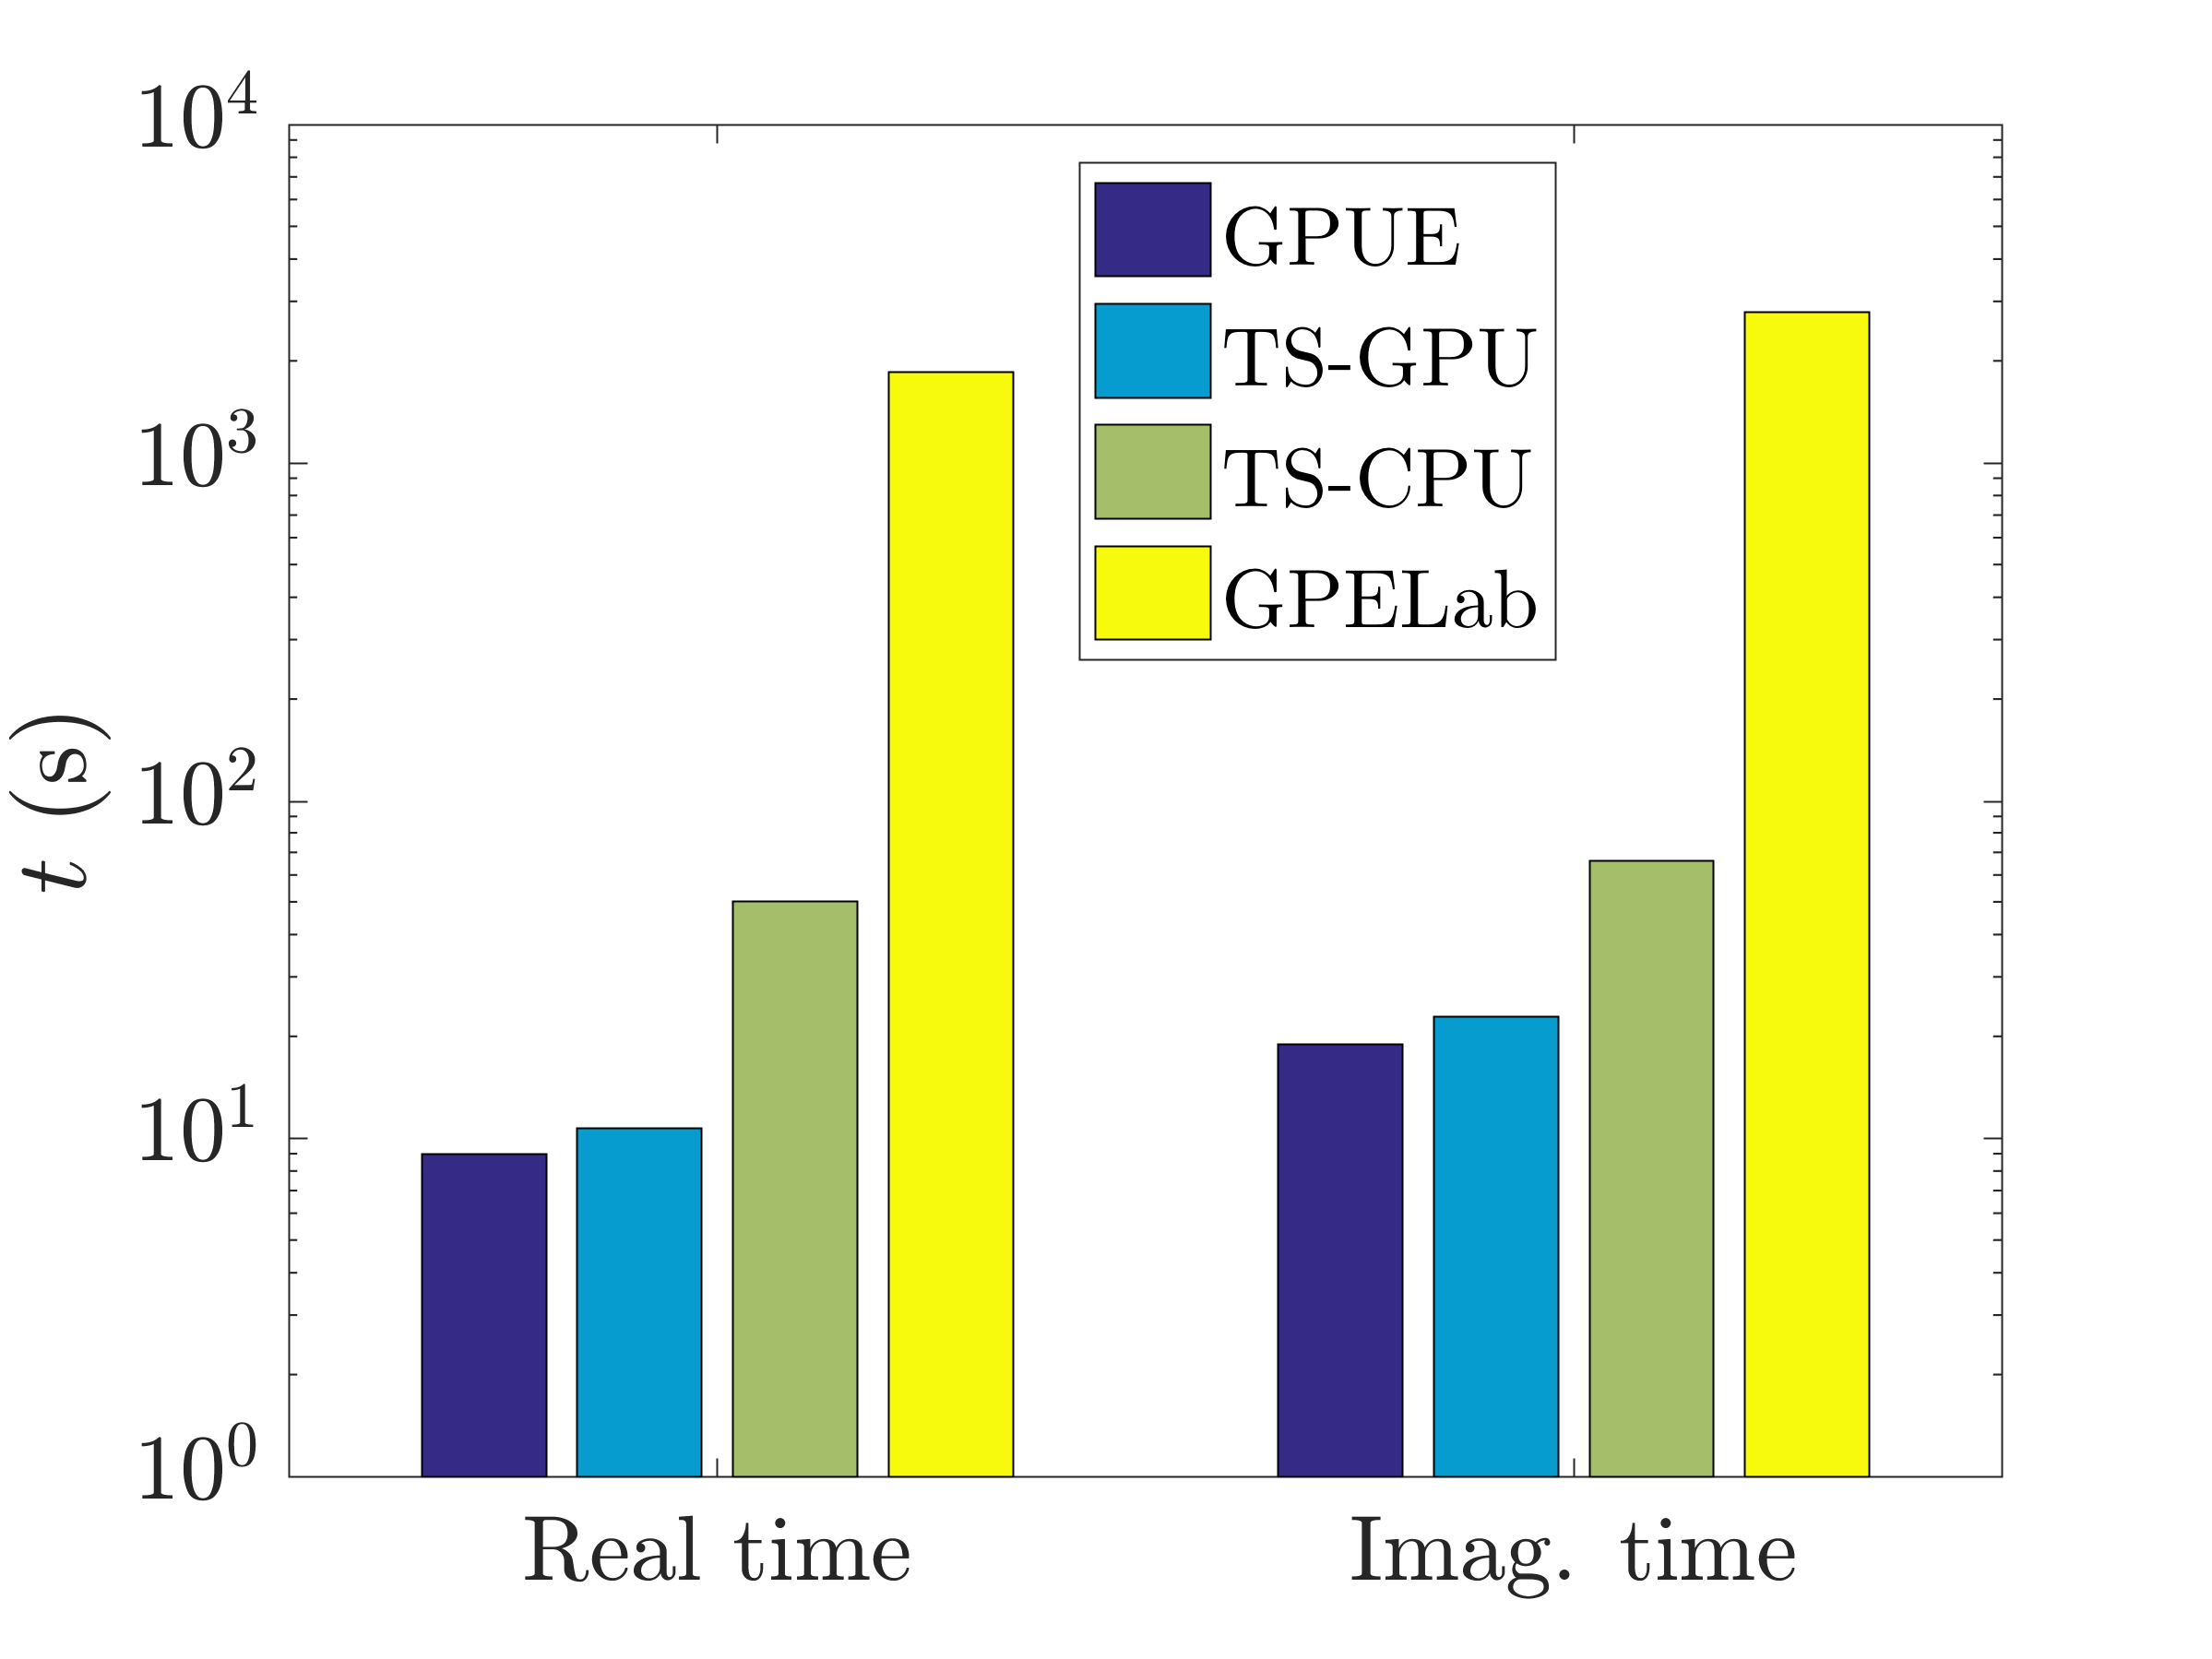
\includegraphics[width=0.7\textwidth,]{ch3_numerics/GPUEvsTS.png}
    \caption{Performance comparison of GPUE and other GPE simulation packages. Data adapted from [wittek url].}
    \label{fig:gpuevsts}
\end{figure}

A simplified sequence and state diagram combination is given in Fig.~\ref{gpue_seq} which describes the operating process for GPUE.

\begin{figure}[h]
    \centering
        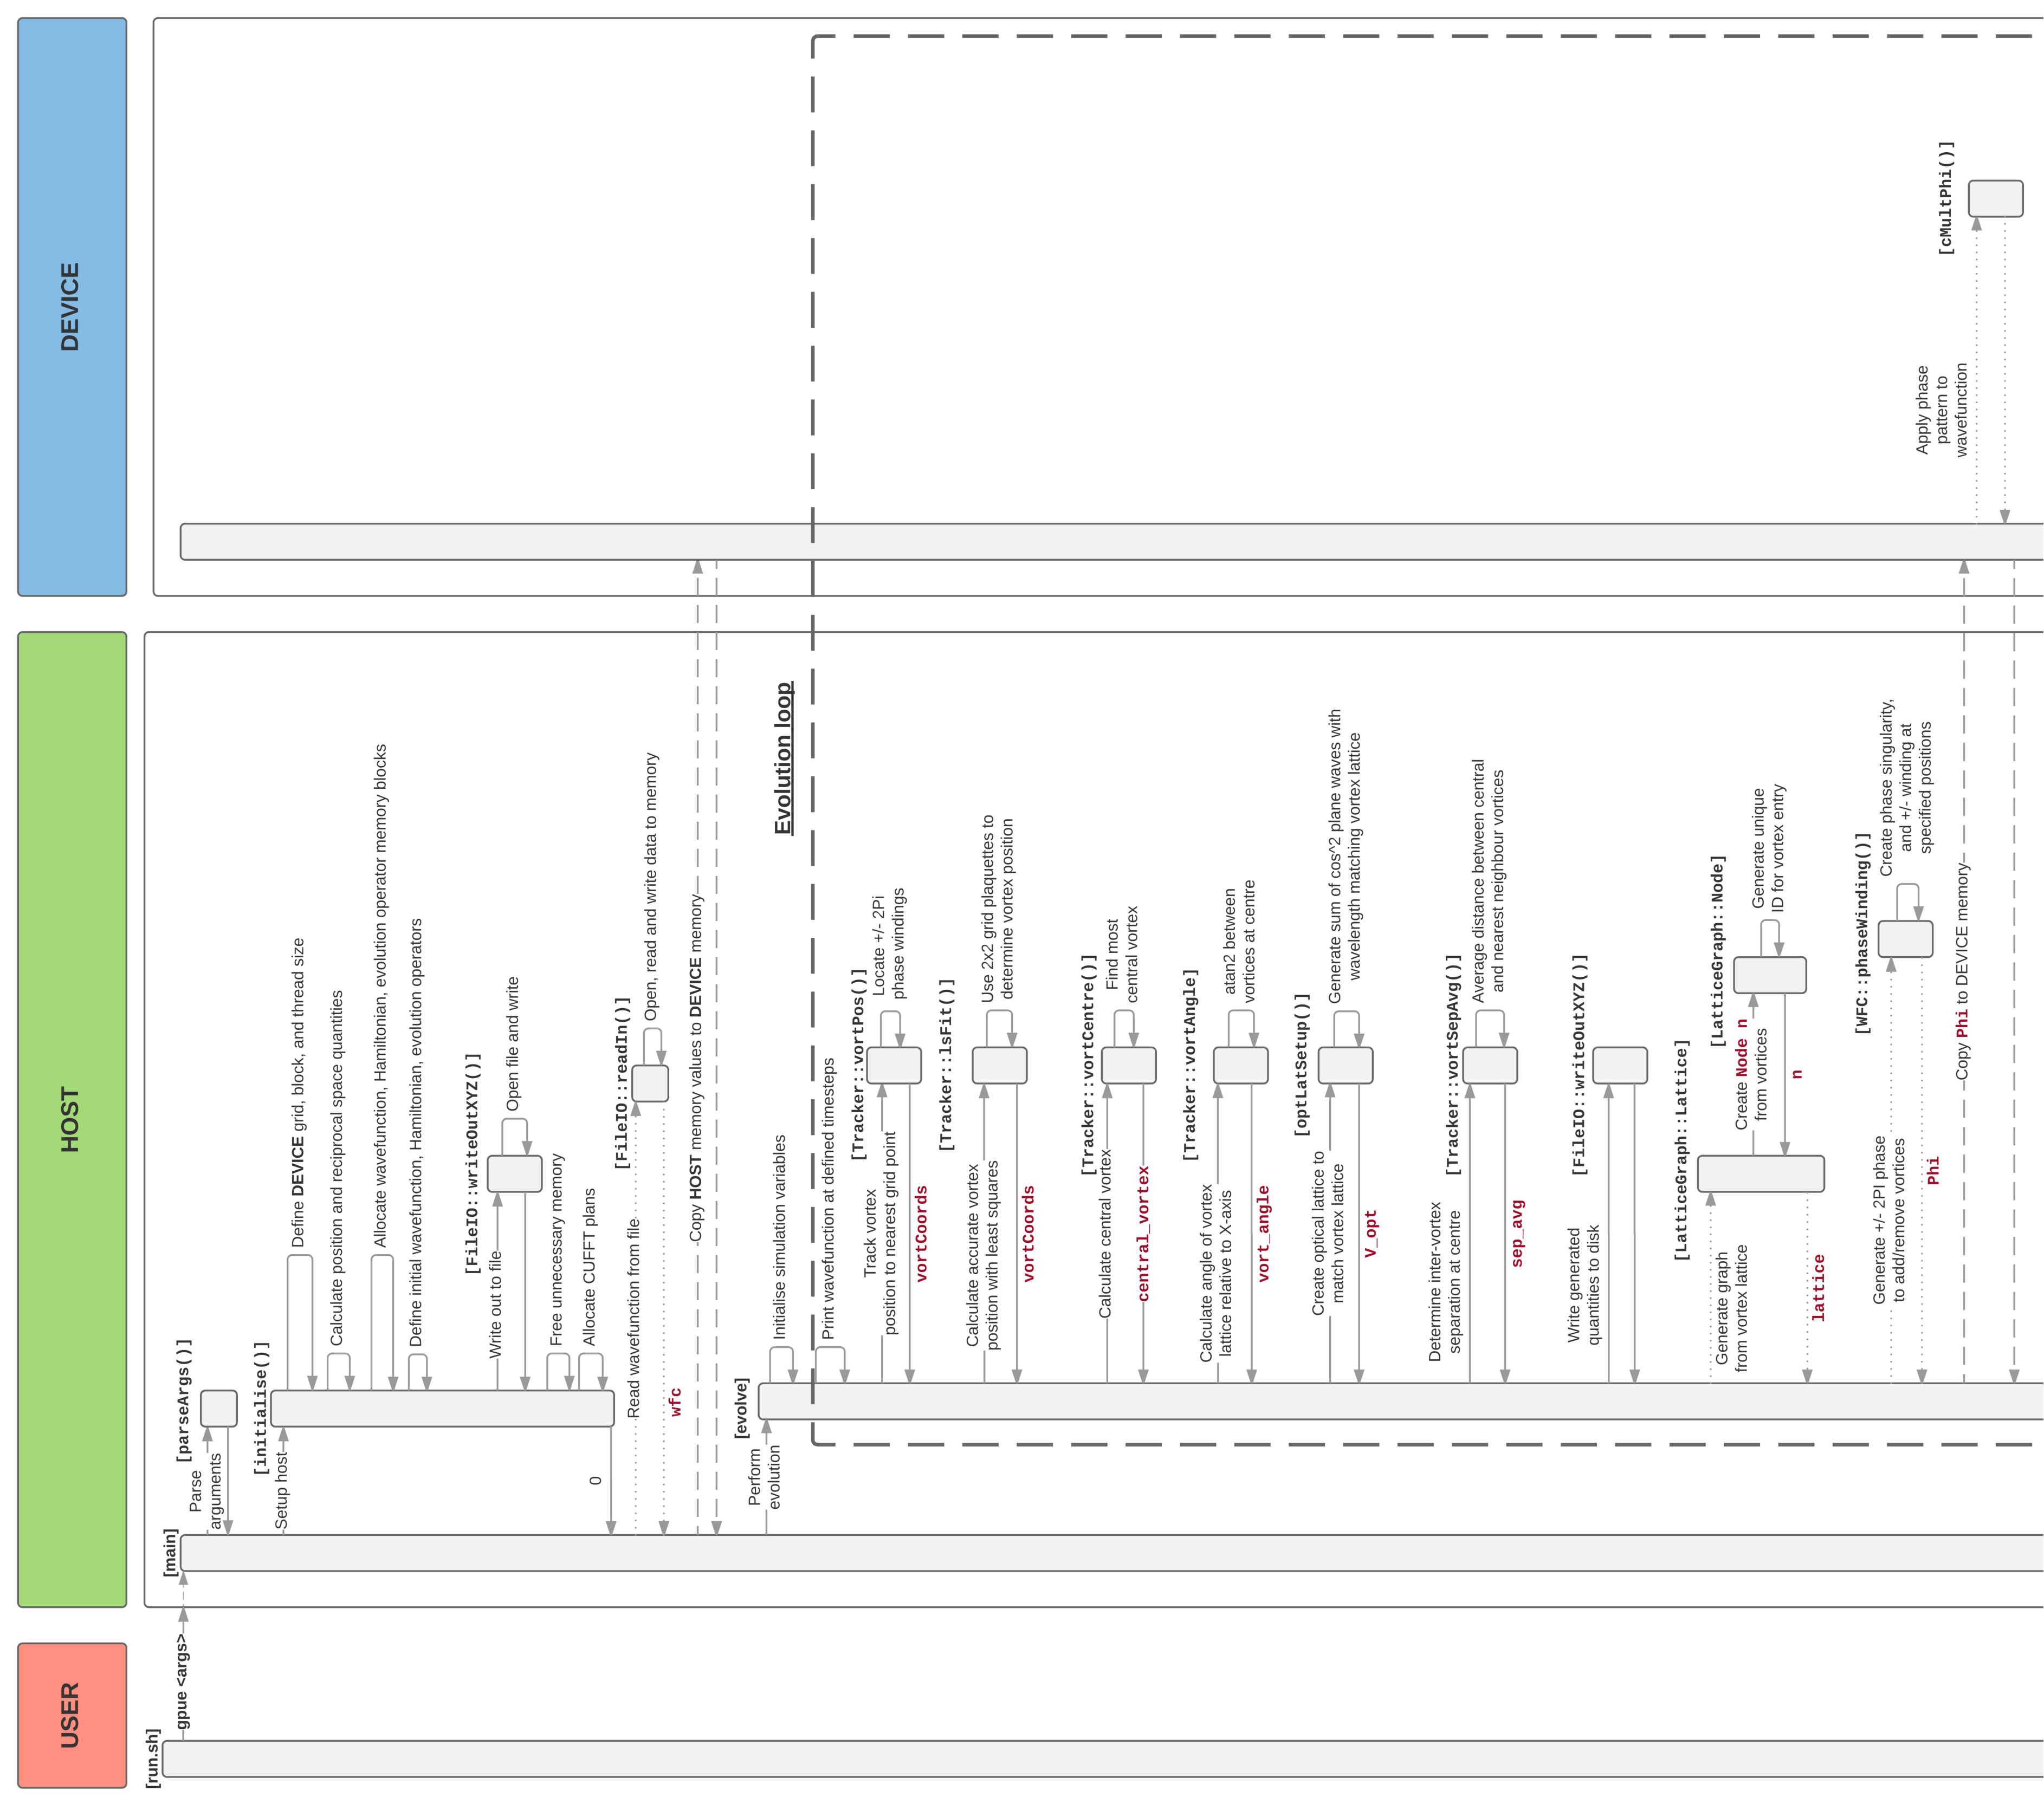
\includegraphics[height=\textwidth,angle=270]{ch3_numerics/GPUE_Seq1}
    \caption{Simplified combined sequence and state diagram for GPUE operation (1 of 2).}
    \label{fig:gpue_seq}
\end{figure}
\begin{figure}[h]
    \centering
        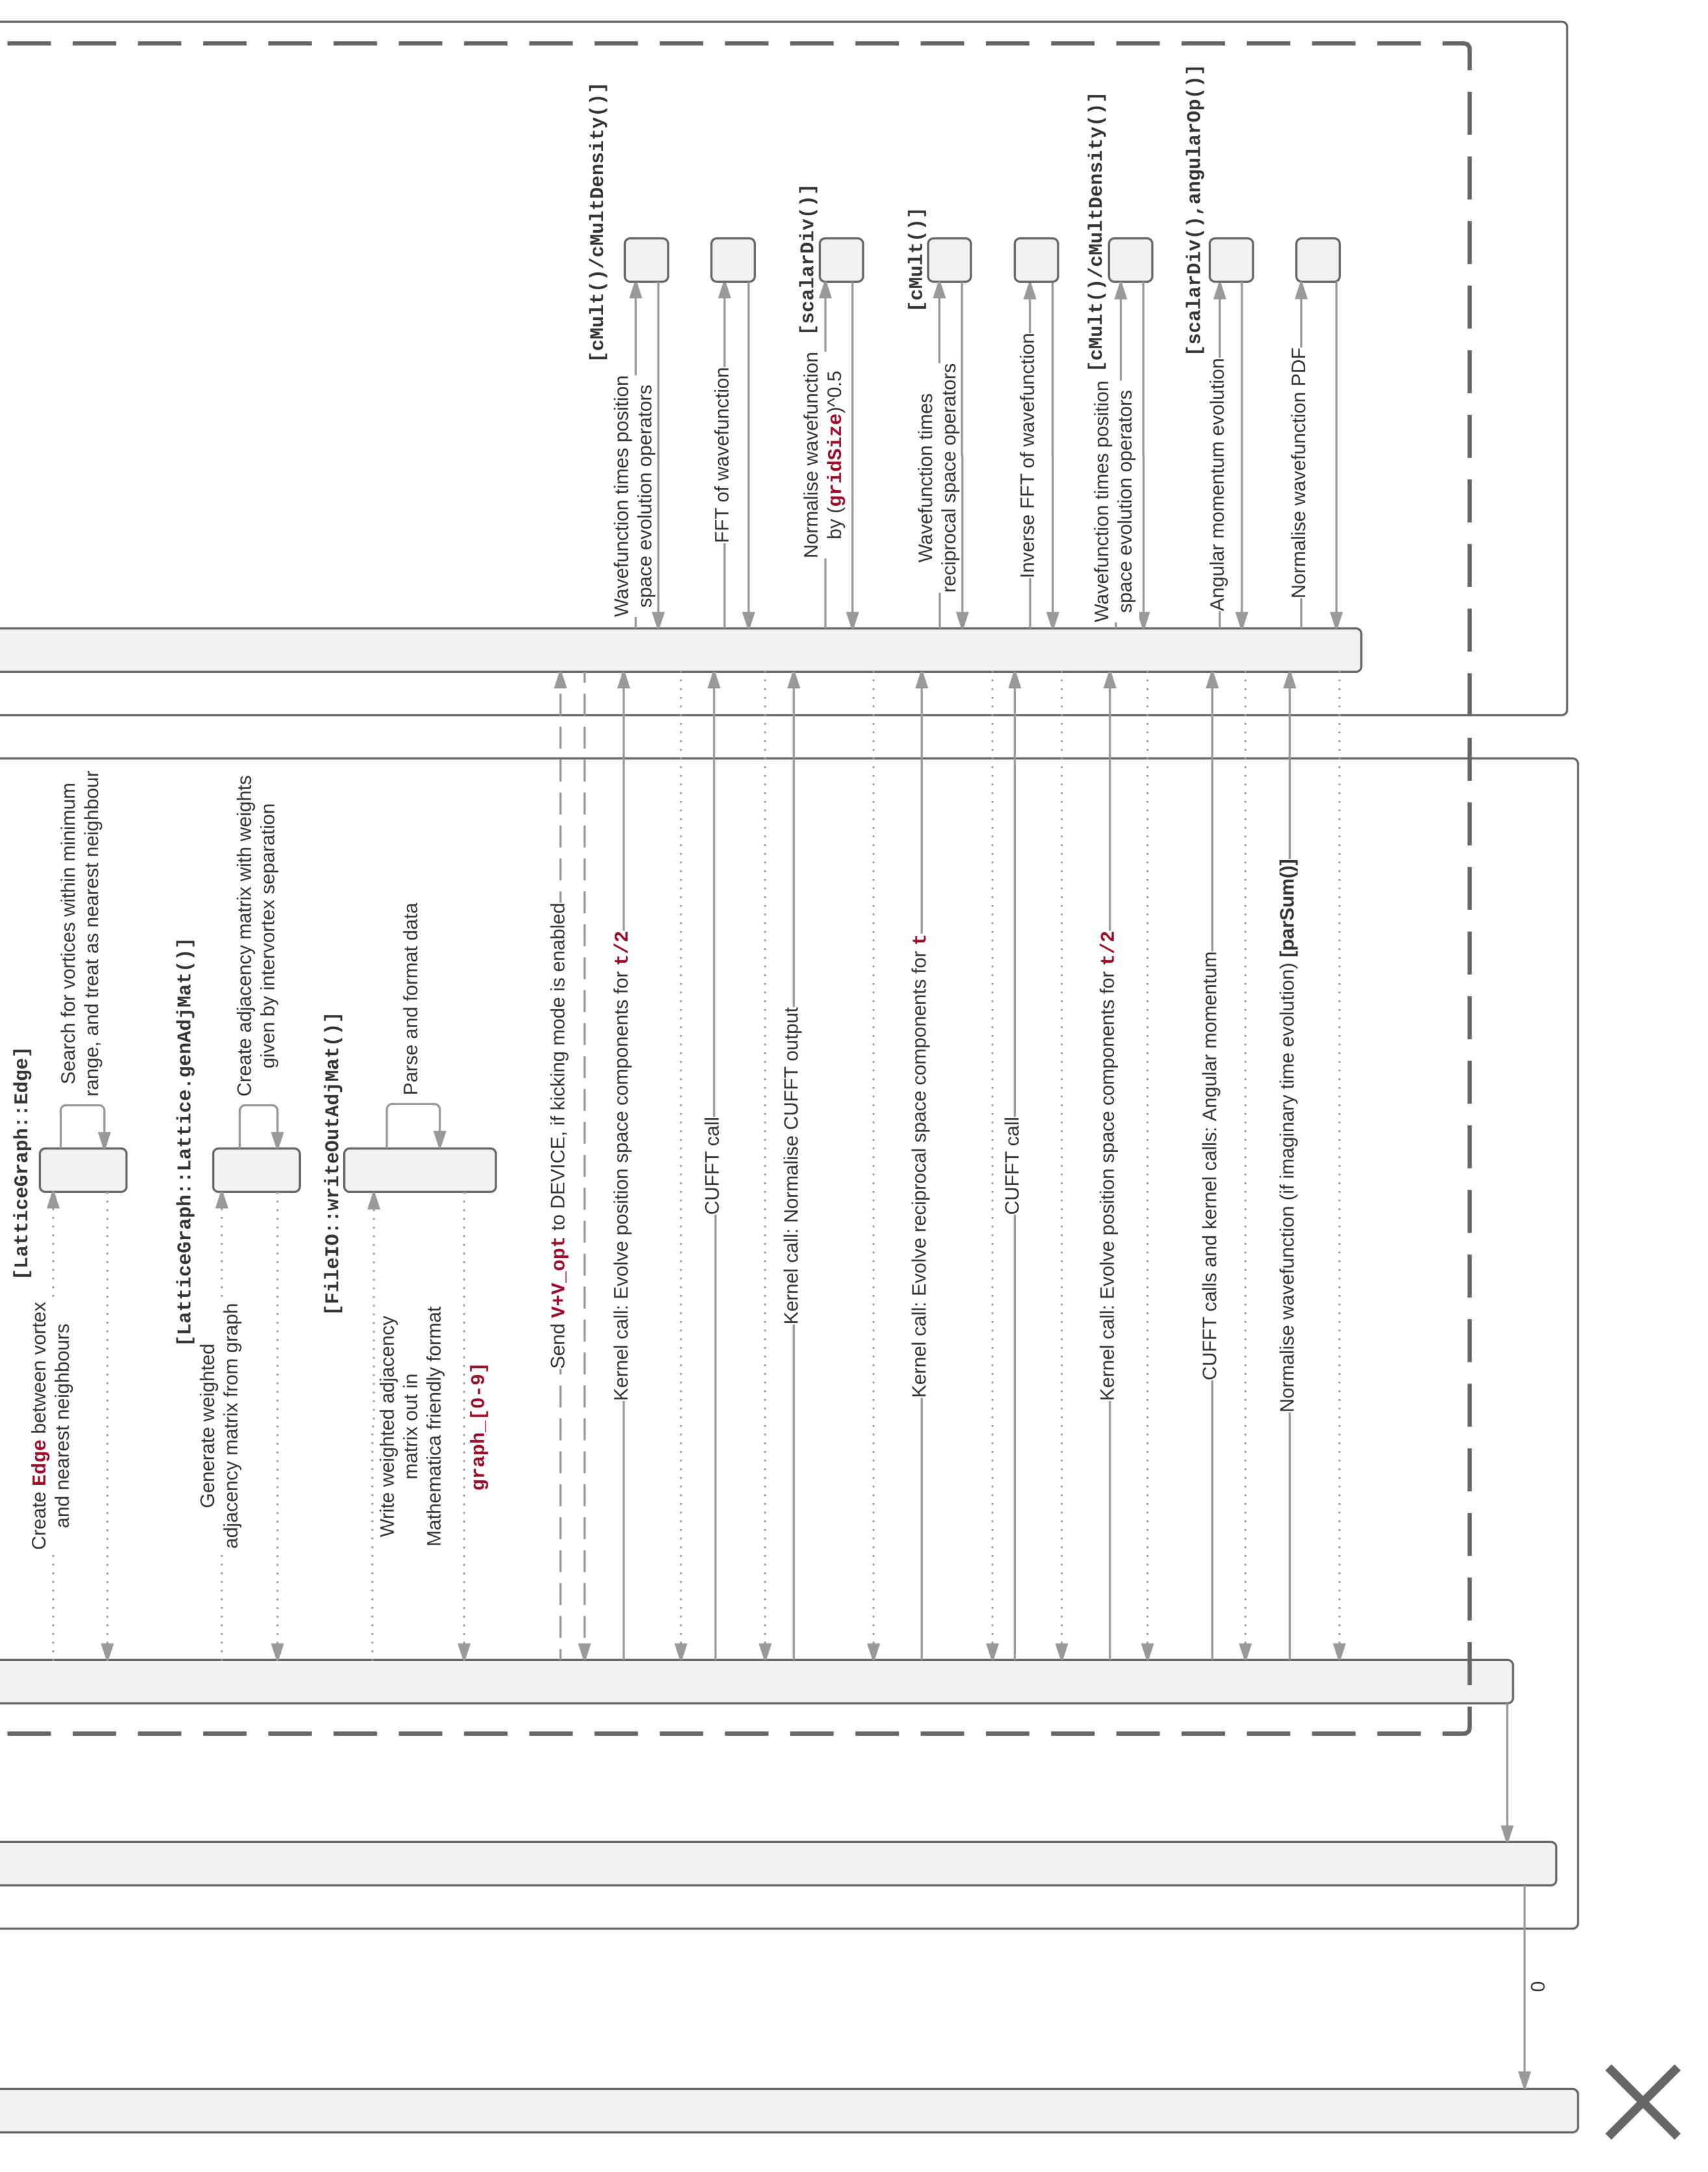
\includegraphics[height=\textwidth,angle=270]{ch3_numerics/GPUE_Seq2}
    \caption{Simplified combined sequence and state diagram for GPUE operation (2 of 2).}
    \label{fig:gpue_seq}
\end{figure}
